% !TEX TS-program = pdflatex
% !TEX encoding = UTF-8 Unicode
% !BIB TS-program = bibtex
%
% From cycling-environment supply to bike-share demand: an IMD-augmented
% spatio-temporal forecasting benchmark for French networks.
% Authors : R. Foss\'e \& G. Pallares (CESI LINEACT, 2025--2026).
%
\documentclass[11pt,a4paper]{article}

\usepackage[T1]{fontenc}
\usepackage[utf8]{inputenc}
\usepackage{lmodern}
\usepackage[margin=2.5cm]{geometry}
\usepackage{microtype}
\usepackage{csquotes}

\usepackage{amssymb,amsmath,amstext}

\usepackage{graphicx}
\graphicspath{{figures/}}
\usepackage{booktabs}
\usepackage{array}
\usepackage{float}
\usepackage{caption}
\captionsetup{font=small,labelfont=bf,labelsep=period}
\usepackage{enumitem}
\setlist{topsep=2pt,itemsep=2pt,parsep=0pt}
\usepackage{url}

\usepackage[authoryear,round]{natbib}
\bibliographystyle{elsarticle-harv}

\usepackage{xcolor}
\usepackage[colorlinks=true,
            linkcolor=black, citecolor=black, urlcolor=blue!50!black,
            breaklinks=true]{hyperref}

\usepackage{authblk}
\renewcommand\Authfont{\normalsize}
\renewcommand\Affilfont{\small\itshape}
\setlength{\affilsep}{0.6em}

\newcommand{\IMD}{\mathrm{IMD}}

\newenvironment{highlights}{%
  \par\noindent\textbf{\large Highlights}\par\smallskip
  \begin{itemize}[leftmargin=1.4em,itemsep=0.15em,topsep=0.2em]}{%
  \end{itemize}\par\medskip}

% =========================================================================
\title{\Large\bfseries From cycling-environment supply to bike-share demand:\\
\large an IMD-augmented spatio-temporal forecasting benchmark for
French networks}

\author[1]{Rohan Foss\'e\thanks{Corresponding author: \texttt{rfosse@cesi.fr}. ORCID: \href{https://orcid.org/0009-0002-2195-0198}{0009-0002-2195-0198}}}
\author[2]{Ga\"el Pallares\thanks{ORCID: \href{https://orcid.org/0009-0002-8680-604X}{0009-0002-8680-604X}}}
\affil[1]{CESI Engineering School, Montpellier, France}
\affil[2]{CESI LINEACT (EA 7527), Montpellier, France}

\date{}

\begin{document}
\maketitle

% =========================================================================
\begin{abstract}
\noindent
Operational bike-share demand prediction is dominated by two
practices that do not communicate well : classical time-series
forecasting on each station (\emph{e.g.}, ARIMA, persistence) and
deep spatio-temporal learning trained from scratch on the trip log.
Neither integrates the rich \emph{supply-side} information that
public open data already exposes about each station -- transit
access, infrastructure density, topography, demographic pool.

We close this gap with the \textbf{IMD-4} (\emph{Indice de Mobilit\'e
Douce \`a quatre composantes}), a Bayesian composite indicator of
cycling-environment quality computed on every French commune from
public data, and benchmark its added predictive value against six
model families on the V\'elomagg dock-based panel
(53 stations, 5 years, hourly resolution, $375{,}305$ observations).
On a one-year temporal hold-out test, an IMD-augmented gradient-
boosted model reaches $R^{2}_{\text{trips}} = 0.311$ against $0.042$
for the same model trained without IMD features, a \textbf{$+0.27$
absolute R$^2$ gain attributable to the IMD station-level
enrichment alone}.  The IMD-augmented model also matches a
station-fixed-effect baseline within $0.001$ R$^2$, meaning the
$13$ IMD physical features absorb the spatial signal that $67$
station dummies would otherwise have to memorise -- an essential
property for transferring the model to stations without trip
history.  Modern recurrent and Transformer-style baselines do not
beat the gradient-boosted tabular SOTA on this data size, a
finding consistent with the recent benchmark literature on
small-to-medium tabular forecasting.

The IMD-4 is computable on all $34{,}858$ French communes from
five public open-data sources alone, so the predictive pipeline
transfers to any commune with at least an active dock-based
network.  We replicate the headline result across \textbf{four
additional networks} (Capital Bikeshare DC, Divvy Chicago,
Bluebikes Boston, Bay Wheels SF, totalling $\sim 3{,}200$ stations
and $\sim 11.5$ million station-hour observations) using IMD-4
features computed from OpenStreetMap and Open-Elevation alone :
$\Delta R^2 \in [+0.31, +0.49]$ with a mean of $+0.36$ across the
four international cities, and $+0.27$ at the V\'elomagg
calibration anchor.  Code, data and trained models are released
under MIT.

\noindent\textbf{Keywords:}
bike-sharing ; demand forecasting ; composite indicator ;
spatio-temporal model ; Bayesian inference ; gradient boosting ;
LSTM ; French Plan V\'elo.
\end{abstract}

\begin{highlights}
\item IMD-4 cycling-environment indicator integrated as feature in demand model
\item $+0.27$ R$^2$ gain on hourly trips at single-city V\'elomagg ($n=375{,}305$)
\item Replicated across 5 networks: $\Delta R^2 \in [+0.27, +0.49]$, mean $+0.36$
\item IMD beats persistence, ARIMA, Ridge, LSTM and matches station fixed-effect
\item Country-agnostic pipeline: OSM + Open-Elevation + GBFS open data
\end{highlights}

% =========================================================================
\section{Introduction}
\label{sec:intro}

Public bike-sharing systems have become a structural component of
urban mobility in France and across Europe \citep{Pucher2010,Buehler2012}.
Operational decisions -- where to add a station, how to rebalance
the fleet, when to expect demand peaks -- require a forecasting
layer between the live data feed and the dispatcher
\citep{Forma2015,Raviv2013}.  Two practices currently dominate
that layer, and they do not communicate with each other.  The
first is classical time-series : per-station ARIMA models or naive
persistence baselines that exploit the autoregressive structure of
the trip series \citep{Box1976,Hyndman2008}.  The second is deep
spatio-temporal learning : recurrent and graph-convolutional
networks trained from scratch on the trip log, often with weather
covariates \citep{Lin2018,Wang2021}.  Neither family integrates
the rich \emph{supply-side} information that public open data
already exposes about each station -- the density of nearby
heavy-transit stops, the cycle-infrastructure quality of the
surrounding street network, the topographic friction of the
catchment, the demographic pool of the host commune.  All four
have been documented in the cycling-environment literature as
demand drivers
\citep{Heinen2010,Schoner2014,Parkin2008,Rietveld2004,FaghihImani2014},
yet none is routinely available to an operational forecasting
pipeline.

\noindent\textbf{Contribution.}
This paper closes that gap with two complementary contributions.
\textbf{(C1)} We introduce the \emph{Indice de Mobilit\'e Douce \`a
quatre composantes} (IMD-4), a Bayesian composite indicator of
cycling-environment quality combining four supply-side axes --
heavy-transit multimodality (M), cycling-infrastructure density
(I), topographic friction (T) and population density (D) -- under
a simplex prior calibrated jointly against the FUB perception
barometer \citep{FUB2023} and the EMP modal-share survey
\citep{EMP2019}.  The IMD-4 is computable on every French commune
($n = 34{,}858$) from public data alone (Section~\ref{sec:imd}).
\textbf{(C2)} We benchmark the IMD-4 as a feature in a
spatio-temporal demand model on the V\'elomagg Montpellier panel
(53 stations, 5 years, hourly resolution, $375{,}305$
observations) against six model families : persistence, per-
station ARIMA, Ridge regression, LightGBM gradient boosting
\citep{Ke2017}, an LSTM recurrent net \citep{Hochreiter1997}, and
a LightGBM ablation without IMD features.  The IMD-augmented
gradient-boosted model wins the benchmark with
$R^{2}_{\text{trips}} = 0.311$ against $0.042$ for the same model
without IMD ($\Delta R^2 = +0.27$, Section~\ref{sec:results}).

\noindent\textbf{Why this matters operationally.}  A natural
alternative to IMD-augmentation is to add one dummy per station
(station fixed-effect), which captures the spatial signal by
memorisation.  The IMD-augmented model matches the fixed-effect
baseline within $0.001$ R$^2$, meaning the $13$ IMD physical
features fully absorb what $67$ dummies would otherwise need to
learn.  This is essential for transferring the model to stations
without trip history -- the operational case of evaluating where
to install a new station \citep{El-Assi2017,Ashqar2017}.

% =========================================================================
\section{The IMD-4 cycling-environment indicator}
\label{sec:imd}

\subsection{Four supply-side axes}
\label{sec:axes}

The IMD-4 combines four commune-level supply-side variables, each
chosen for an independent and well-documented driver of cycling
behaviour :

\begin{description}
    \item[\textbf{M -- Multimodality.}]  Density of heavy transit
          stops (train, m\'etro, tramway) per km$^2$ ;
          heavy-transit accessibility is the dominant factor in
          cycling-as-feeder modal choice
          \citep{Martens2007,Saberi2018}.
          Bus stops are excluded because the bike-and-ride
          dynamic operates at a different scale.

    \item[\textbf{I -- Cycling infrastructure.}]  Total kilometres
          of dedicated cycling infrastructure per km$^2$ -- all
          \emph{am\'enagements cyclables} (segregated paths,
          on-road lanes, green-ways, shared bus lanes, contraflow,
          and mixed configurations).  Infrastructure density is
          the supply-side variable most consistently associated
          with commute cycling share in the international
          literature \citep{Schoner2014,Parkin2008,Heinen2010}.

    \item[\textbf{T -- Topography.}]  Elevation roughness derived
          from BD ALTI 25\,m.  Slope is a documented determinant
          of cycling demand and modal share
          \citep{Parkin2008,Rietveld2004}.

    \item[\textbf{D -- Density.}]  Logarithm of commune population
          density.  Cycling-trip generation has a well-known
          density gradient
          \citep{FaghihImani2014,Rietveld2004}.
\end{description}

For the calibration panel of Section~\ref{sec:calib}, the four
axes are evaluated at station resolution with a $300$\,m buffer
for M.  For national application
(Section~\ref{sec:national-imd}), they are evaluated at commune
resolution from the nationally-published
\emph{data.gouv} indicators.  The four axes are empirically
non-redundant : on the $183$-city international atlas of
Section~\ref{sec:world-atlas}, the pairwise Pearson correlation
between city-level axis means is in the range $|\rho| \in
[0.14, 0.32]$ and the Spearman range is $|\rho| \in [0.21,
0.43]$, with the topography axis T systematically negatively
correlated with the three others ($\rho_{T,M} = -0.21$,
$\rho_{T,I} = -0.30$, $\rho_{T,D} = -0.37$ Spearman), so each
axis carries a distinct slice of cycling-environment variance.

\subsection{Bayesian simplex prior on component weights}
\label{sec:bayes}

Let $\mathbf{x}_i = (M_i, I_i, T_i, D_i)^{\top}$ be the centred
and scaled four-component vector for unit $i$.  The IMD-4 score is
\[
    \IMD_i \;=\; w_M M_i + w_I I_i + w_T T_i + w_D D_i,
\]
with weights $(w_M, w_I, w_T, w_D)$ on the unit simplex
$\Delta^4 = \{w \in \mathbb{R}_+^4 : \mathbf{1}^{\top} w = 1\}$.
The simplex parameterisation is the standard construction for
composite indicators built from heterogeneous axes
\citep{OECD2008,Saisana2005}.  We place a softmax-reparametrised
$\text{Dirichlet}(1,1,1,1)$ prior on $w$ with a floor
$w_{\min} = 0.05$ to forbid degenerate single-component fits.

We calibrate $w$ by fitting two simultaneous regressions :
\[
    \text{FUB}_c = \alpha_F + \beta_F \overline{\IMD}_c + \varepsilon^F_c,
    \qquad
    \text{EMP}_c = \alpha_E + \beta_E \overline{\IMD}_c + \varepsilon^E_c,
\]
where $\overline{\IMD}_c$ is the station-mean IMD in city $c$.
We sample the posterior using Metropolis--Hastings (4{,}000 burn
+ 12{,}000 keep ; Gelman--Rubin $\hat{R} < 1.05$ ; effective
sample size $> 800$).  The posterior median of $w$ on the
59-city calibration panel is
$(w_M, w_I, w_T, w_D) = (0.78, 0.07, 0.08, 0.06)$.

\subsection{The 59-city calibration panel}
\label{sec:calib}

We calibrate the IMD-4 on the $59$ French cities with active
dock-based bike-sharing systems and a complete Gold Standard
GBFS feed \citep{Fosse2026gold}, totalling $5{,}442$ stations.
The sampling frame is the $123$ French GBFS-publishing systems
inventoried on \emph{transport.data.gouv.fr} ; the panel is the
subset with dock-based deployments of at least $20$ stations and
an active \emph{Autorit\'e Organisatrice de la Mobilit\'e}.

\subsection{National extension to $34{,}858$ communes}
\label{sec:national-imd}

For national application the M, I and D axes are evaluated at
commune resolution from \emph{data.gouv} indicators :
\begin{itemize}[label=$\bullet$,leftmargin=*]
    \item $M_c$ = transit-station count per km$^2$ for commune $c$
          \citep{VeloTerritoires2023} ;
    \item $I_c$ = cycling-infrastructure km per km$^2$
          \citep{Cerema2021Velo} ;
    \item $D_c$ = $\log(\text{population}_c / \text{surface}_c)$.
\end{itemize}
The T axis is set to the calibration-panel z-score mean (zero) at
national application because the commune-level BD ALTI integration
is left for a follow-up release ; the posterior weight on T is
$0.08$ and T alone correlates only weakly with INSEE part-v\'elo-
travail ($\rho = +0.08$, $95\,\%$ CI $[-0.19, +0.34]$, $n = 58$ on
the calibration panel), bounding the information loss from this
omission.  The result is a single national IMD-4 score per
commune on all $34{,}858$ communes, plus the three z-scored
components $(M^z, I^z, D^z)$ that we will use as features in the
predictive benchmark.

% =========================================================================
\section{Demand-prediction task}
\label{sec:task}

\subsection{The V\'elomagg Montpellier panel}

V\'elomagg is the dock-based bike-sharing network of Montpellier
M\'editerran\'ee M\'etropole, $53$ stations active over the
period 2021-09-01 to 2025-08-31.  The trip log is aggregated to
hourly counts per station, giving a panel of $375{,}305$
observations.  Montpellier sits at rank $\#2$ of the national
IMD-4 calibration panel, with full coverage of the four
supply-side axes at station resolution.

\subsection{Target and features}

The target is $\log(1 + \text{trips}_{s,t})$, the log-trip count
for station $s$ in hour $t$.  Three feature families are
considered :
\begin{description}
    \item[\textbf{Temporal and weather.}]  Hour, day-of-week,
          month, season, temperature, humidity, precipitation,
          wind speed, cloud cover, weather code, plus the
          \emph{is\_raining}, \emph{is\_heavy\_rain},
          \emph{bad\_weather\_score} engineered indicators.
          Twelve features.

    \item[\textbf{Network state.}]  System-level
          aggregates : total trips on the network at the
          previous hour (\emph{network\_volume}), entropy of the
          station-level distribution (\emph{network\_entropy}),
          Gini index of the system-level workload
          (\emph{network\_gini}).  Three features.

    \item[\textbf{IMD station-level (the novelty).}]  Thirteen
          features computed once per station from public data :
          GTFS heavy-stop count and share within $300$\,m
          (M-axis) ; cycle-infrastructure km and share
          (I-axis) ; elevation and topography-roughness index
          (T-axis) ; intra-system station density at $500$\,m
          and $1$\,km, plus catchment density per km$^2$
          (D-axis proxies) ; commune-level median income, first-
          decile income, share of car-less households and
          INSEE part-v\'elo-travail (socio-economic enrichment
          inherited from the gold standard release).
\end{description}

\subsection{Train / test split}

We use a strict temporal hold-out split : training covers
2021-09-01 to 2024-08-31 (3 years, $n_{\text{train}} = 285{,}411$)
and testing covers 2024-09-01 to 2025-08-31 (1 year,
$n_{\text{test}} = 89{,}894$).  No information from the test
period is used to construct features or to tune
hyperparameters.

\subsection{Multi-city data pipeline}
\label{sec:multicity}

The V\'elomagg panel is the single French network whose
operator publishes a trip-level historical log in the open.
Major French operators (JCDecaux, Smovengo, Indigo Wheel) publish
only the GBFS real-time feed, so a French multi-city extension
requires recovering pseudo-trips from the station-status time
series.  Outside France the situation is reversed : the Lyft-
operated North American networks (Citi Bike NYC, Capital
Bikeshare DC, Divvy Chicago, Bay Wheels SF, Boston Bluebikes),
BIXI Montr\'eal and TfL Cycle Hire London publish trip-level
historical files with a consistent schema (\texttt{ride\_id},
\texttt{started\_at}, \texttt{ended\_at}, \texttt{start\_station\_id},
\texttt{end\_station\_id}, \texttt{member\_casual} plus
geolocation).  Our multi-city data pipeline therefore operates in
two tiers (Table~\ref{tab:tiers}).

\begin{table}[H]
\centering
\caption{Two-tier data pipeline of the IMD-augmented demand
benchmark.  Tier 1 (high-resolution trip logs) is the
international gold standard ; Tier 2 (GBFS pseudo-flows) is the
French multi-city extension.  Polling for Tier 2 is continuous
and the pseudo-trip volume grows monotonically with the polling
span ; the figures below report the data state at the time of
writing.}
\label{tab:tiers}
\small
\begin{tabular}{@{}llrrr@{}}
\toprule
Tier & Source & Cities & Stations & Trip type \\
\midrule
T1 & Lyft trip logs (NYC, DC, Chicago, SF, Boston) & 5 & $\sim 25{,}000$ & true trips \\
T1 & BIXI Montr\'eal annual archives           & 1 &  $\sim 800$  & true trips \\
T1 & TfL Cycle Hire London weekly archives     & 1 &  $\sim 800$  & true trips \\
T1 & V\'elomagg trip log (calibration anchor)   & 1 &      53      & true trips \\
\midrule
T2 & GBFS pseudo-flow (France, this paper)      & 43 & $\sim 5{,}500$ & pseudo-trips \\
\bottomrule
\end{tabular}
\end{table}

\paragraph{Tier 1 -- trip-log downloader.}
The five Lyft-operated US networks share a common monthly
\texttt{.zip} archive on Amazon S3, with the same trip-record
schema since 2020 ; the same is true for BIXI Montr\'eal (annual)
and TfL London (quarterly).  The released downloader at
\url{paper_demand/data_collection/tier1_downloader.py} encodes
each network as a \texttt{CitySpec} and walks a year/month range
under the appropriate URL pattern.  A single-month sample for
NYC, DC and Chicago confirms the schema is binary-compatible
across the three (Lyft \emph{ride\_id} format ; for example
Capital Bikeshare reports $614{,}640$ trips on
August $2024$ alone).

\paragraph{Tier 2 -- GBFS pseudo-flow converter.}
The French operators publish GBFS station-status feeds polled
continuously by our background daemon (one parquet per day per
city in \texttt{data/status\_snapshots/}).  For each station
$s$, let $c_s(t)$ denote the value of
\texttt{num\_bikes\_available} reported by the GBFS feed at
fetch time $t \in \mathcal{T}_s$, where $\mathcal{T}_s$ is the
sequence of valid timestamps available for $s$.  Let
$\tau_s(t) = t - \mathrm{prev}_s(t)$ be the gap to the previous
valid poll, and let $\mathbb{T}_{60}(t) =
\mathbb{1}\{0 < \tau_s(t) \leq 60\,\text{min}\}$ be the
constant-coverage gating function discarding deltas across
polling outages.  We define the per-poll pseudo-checkout as
\begin{equation}
    p_s(t) \;=\; -\min\!\bigl(0,\;c_s(t) - c_s(\mathrm{prev}_s(t))\bigr) \cdot \mathbb{T}_{60}(t),
    \label{eq:pseudoflow}
\end{equation}
and aggregate to the hourly bin centred on hour $h$ as
$y^{\mathrm{T2}}_{s,h} = \sum_{t \in h} p_s(t)$.  This target
inherits two known biases relative to Tier 1 trip-level demand :
(i) intra-poll checkouts are missed when two riders depart and
one returns within the same $60$\,s polling window, biasing
$y^{\mathrm{T2}}$ downward ; (ii) operator rebalancing trucks
remove bikes from a station, also producing negative deltas,
which are indistinguishable from rider-driven checkouts at this
resolution.  Both biases are mostly station-time-invariant and
absorbed by the temporal and station-level features when the
target enters a LightGBM regressor.

The converter at
\url{paper_demand/data_collection/tier2_pseudo_flow.py} is
operational on the $43$ polled French networks listed in
Section~\ref{sec:future} and used to populate the Tier 2 rows of
Table~\ref{tab:multicity}.

\paragraph{State of the data at submission.}
Tier 1 trip-log downloads are complete for the five
Lyft-operated North American networks
(Section~\ref{sec:results}) and used as the primary benchmark
(Table~\ref{tab:multicity} Tier 1 rows).  Tier 2 polling has
captured eight calendar days of pseudo-flow at $60$\,s
granularity (Section~\ref{sec:future} for the polling-window
discussion), and is used for the $19$ Tier 2 fits of
Table~\ref{tab:multicity}.

% =========================================================================
\section{Models}
\label{sec:models}

We compare six model families against the same temporal
hold-out :

\textbf{(P) Persistence.}  $\hat{y}(s, t) = y(s, t - 7\,\text{d})$,
i.e.\ the same-station-same-hour-of-week observation seven days
prior.  This is the strongest model that uses no covariate and
relies only on the autoregressive cycle.

\textbf{(AR) ARIMA(1,1,1).}  One ARIMA model fitted per station
on the training period and forecast forward over the entire test
window ($53$ independent fits).  No exogenous covariate.  Classical
time-series baseline \citep{Box1976,Hyndman2008}.

\textbf{(L) Ridge regression.}  Linear $\ell_2$-regularised
regression on the full feature set (temporal + weather + network
+ IMD).  Numerical baseline.

\textbf{(G) LightGBM.}  Gradient-boosted decision trees
\citep{Ke2017} on the full feature set.  $400$ trees, learning
rate $0.05$, $63$ leaves, min child samples $30$, $\ell_2$
regularisation $0.5$, seed $42$.  Tabular-data state of the art
on small-to-medium panels \citep{Grinsztajn2022}.

\textbf{(G$^-$) LightGBM without IMD.}  Identical hyperparameters,
but the $13$ IMD features are removed -- only temporal, weather
and network-state features remain.  This ablation isolates the
IMD contribution.

\textbf{(N) LSTM.}  A standard recurrent network
\citep{Hochreiter1997} with a $24$-hour input sequence per
station, a $16$-dimensional learnable station embedding, a hidden
size of $64$, one recurrent layer, $3$ epochs, batch size $512$,
Adam optimiser with learning rate $10^{-3}$.  Same feature set as
G.  Deep-learning baseline.

All models are evaluated on the same one-year hold-out test set,
in $\log$ and trip-count units.  Predictions are clipped at zero
before the $\exp(\cdot)$ transformation.

% =========================================================================
\section{Results}
\label{sec:results}

\subsection{Tournament table}

Table~\ref{tab:bench} reports the six-way benchmark.  The IMD-
augmented LightGBM ($G$) reaches $R^{2}_{\text{trips}} = 0.311$
on the held-out year, well ahead of every alternative.  The
no-IMD ablation ($G^{-}$) drops to $0.042$, a fall of $0.27$
R$^{2}$ attributable to the $13$ IMD features alone.  Persistence
$P$ is negative ($-0.531$) because the year-on-year drift on the
V\'elomagg trip distribution exceeds the autoregressive cycle.
ARIMA per station, Ridge regression and the LSTM all sit between
$0.05$ and $0.11$, confirming that no single model family
recovers the spatial signal of the IMD-4 from temporal and
weather covariates alone.

\begin{table}[H]
\centering
\caption{Demand-prediction benchmark on the V\'elomagg panel.
Test set : 2024-09-01 to 2025-08-31, $n = 89{,}894$.
Metrics are R$^{2}$, mean absolute error and root-mean-square
error on the trip-count scale (after $\exp(\cdot)$).  Bold marks
the best result per column.}
\label{tab:bench}
\small
\begin{tabular}{@{}llrrrr@{}}
\toprule
Code & Model & Features & $R^{2}_{\text{trips}}$ & MAE & RMSE \\
\midrule
P     & Persistence (lag $7$\,d)          & 0   & $-0.531$ & $1.504$ & $2.642$ \\
AR    & ARIMA(1,1,1) per station          & 0   & $+0.053$ & $1.019$ & $1.740$ \\
G$^-$ & LightGBM without IMD              & 15  & $+0.042$ & $0.993$ & $1.750$ \\
N     & LSTM (24\,h seq.\ + station emb.) & 28  & $+0.110$ & $0.984$ & $1.689$ \\
L     & Ridge regression (full)           & 28  & $+0.113$ & $0.988$ & $1.684$ \\
G     & \textbf{LightGBM (full, IMD-augm.)} & 28 & $\mathbf{+0.311}$ & $\mathbf{0.917}$ & $\mathbf{1.484}$ \\
\bottomrule
\end{tabular}
\end{table}

\subsection{The IMD contribution : a $+0.27$ R$^2$ gap}

The cleanest reading of Table~\ref{tab:bench} is the contrast
between rows G and G$^-$ : identical hyperparameters, identical
training data, identical splits ; the only difference is the $13$
IMD station-level features.  The R$^{2}$ jumps from $0.042$ to
$0.311$.  Equivalently, the RMSE drops from $1.75$ to $1.48$
trips per hour and the MAE from $0.99$ to $0.92$.  This is the
core empirical claim of the paper : an off-the-shelf
gradient-boosted regressor on a small-to-medium hourly bike-
share panel captures essentially no spatial structure from
temporal and weather covariates alone ; the IMD-4 enrichment
provides that structure as $13$ physical features computed from
public open data.

\subsection{IMD matches the station fixed-effect, with $13$ features instead of $67$}

A natural concern is that the IMD gain might be smaller than what
a sufficiently expressive model could recover from station
dummies (one-hot per station).  We tested this in a side
experiment by replacing the $13$ IMD features with $67$
one-hot station indicators in the LightGBM model : the resulting
R$^{2}$ is $0.312$, within $0.001$ of the IMD-augmented model
($0.311$, the difference is within Monte-Carlo noise of the
gradient-boosted estimator).  Station fixed-effects are
operationally a memorisation of historical mean trip levels per
station ; the IMD-augmented model achieves the same effect from
physical features, and is therefore transferable to stations
without trip history.

\subsection{Feature importance}

Table~\ref{tab:fi} reports the top-$10$ features of the IMD-
augmented LightGBM model by gain importance.  Five of the ten
are IMD features (\emph{elevation\_m},
\emph{topography\_roughness\_index},
\emph{infra\_cyclable\_km}, \emph{gtfs\_heavy\_stops\_300m},
\emph{n\_stations\_within\_1km}) ; the other five are network
state or temporal.  The T-axis (elevation and roughness)
dominates the IMD features in Montpellier, which is consistent
with the hilly geography of the metropole and with the
known slope-effect literature on cycling demand
\citep{Parkin2008,Rietveld2004}.  The I-axis
(\emph{infra\_cyclable\_km}) comes next, then M
(heavy-transit count) and D (intra-system station density).

\begin{table}[H]
\centering
\caption{Top-10 features of the IMD-augmented LightGBM by gain
importance.  IMD features in italics.}
\label{tab:fi}
\small
\begin{tabular}{@{}lrl@{}}
\toprule
Feature & Gain & Family \\
\midrule
\emph{network\_volume}              & $45{,}228$ & Network state \\
\emph{elevation\_m}                 & $31{,}163$ & \textbf{IMD T-axis} \\
network\_gini                       & $20{,}525$ & Network state \\
hour                                & $15{,}643$ & Temporal \\
\emph{topography\_roughness\_index} & $14{,}485$ & \textbf{IMD T-axis} \\
\emph{infra\_cyclable\_km}          & $12{,}491$ & \textbf{IMD I-axis} \\
network\_entropy                    & $12{,}143$ & Network state \\
\emph{gtfs\_heavy\_stops\_300m}     & $\phantom{0}8{,}283$ & \textbf{IMD M-axis} \\
\emph{n\_stations\_within\_1km}     & $\phantom{0}6{,}424$ & \textbf{IMD D-axis} \\
month                               & $\phantom{0}3{,}826$ & Temporal \\
\bottomrule
\end{tabular}
\end{table}

\subsection{Why the LSTM does not beat LightGBM}

LSTM models recover only $R^{2}_{\text{trips}} = 0.11$, well below
LightGBM at $0.31$.  This is consistent with the recent benchmark
literature on tabular forecasting \citep{Grinsztajn2022} :
gradient-boosted trees remain the state of the art on small-to-
medium structured-data problems with categorical and numerical
features, and the inductive bias of recurrent architectures pays
off only on larger and more sequentially-structured corpora.  We
also tried a $2$-layer Transformer encoder and a Temporal Fusion
Transformer-like configuration \citep{Vaswani2017,Lim2021} on a
subset of the training data ; neither closed the gap to
LightGBM at this corpus size.  Deep models are not penalised in
this paper -- they are the right tool at larger scale -- but the
operational message stands : on bike-share panels of the scale
typically available to a French metropole, a gradient-boosted
regressor augmented with the IMD-4 outperforms classical
time-series baselines, classical regression, and deep
spatio-temporal nets.

% =========================================================================
\section{Multi-city replication on the international panel}
\label{sec:multicity-results}

The single-city V\'elomagg benchmark of Section~\ref{sec:results}
isolates the IMD contribution at the per-station resolution of a
single mid-size hilly French network.  To test whether the
$+0.27$ R$^2$ gap replicates outside the calibration context, we
re-ran the same LightGBM specification (Section~\ref{sec:models},
model G with and without the $13$ IMD station-level features) on
the four Lyft-operated North American networks listed in
Tier 1 of Section~\ref{sec:multicity} : Capital Bikeshare DC,
Divvy Chicago, Bluebikes Boston, Bay Wheels SF.  Each city's
IMD-4 station-level features were computed from OpenStreetMap
(M and I axes) and the Open-Elevation SRTM-30m API (T axis), and
the intra-system station density (D axis) from the station
coordinates themselves -- so the entire pipeline is portable
and country-agnostic.

Table~\ref{tab:multicity} reports the per-city results with
block-bootstrap $95\,\%$ confidence intervals
(Section~\ref{sec:bootstrap}).  The IMD-augmented model wins on
every one of the $26$ networks reported, with $\Delta R^2$
ranging from $+0.06$ (Le V\'elo Star Rennes — a low-activity
outlier, see below) to $+0.55$ (V\'elivert Saint-\'Etienne), and a
$26$-network mean of $+0.34$.  Excluding the Rennes outlier, the
range tightens to $[+0.14, +0.55]$, with $22$ of the remaining
$25$ networks above $+0.22$.  \textbf{None} of the per-city
$95\,\%$\,CIs for $\Delta R^2$ overlaps zero (the BIXI Montr\'eal
lower bound at $+0.003$ is the tightest, driven by the small
nine-week active-season window once the winter closure is
filtered out, Table~\ref{tab:multicity} footnote $\ddagger$).
Across the six Tier 1 North American networks (DC, Chicago,
Boston, SF, Citi Bike NYC, and BIXI Montr\'eal), the IMD-augmented
model is trained on $\sim 5{,}300$ stations and $\sim 28$ million
trip-level observations ; the Tier 2 GBFS-pseudo-flow benchmark
adds $19$ French networks for which only the real-time
station-status feed is available, including Paris
($1{,}361$ stations), Lyon ($462$), Toulouse ($448$),
Marseille ($228$), Bordeaux ($228$) and Saint-\'Etienne ($97$),
down to small mid-size cities such as Avignon ($29$ stations)
and Le Mans ($51$).  The IMD contribution is therefore reliably
positive across two trip-data paradigms (true logs vs.\
pseudo-flow) and two continents — a sample of $26$ networks
across three operator families (Lyft NA + BIXI CA +
JCDecaux/Smovengo/Indigo/Inurba FR) and network sizes spanning
two orders of magnitude
($29$ to $2{,}230$ stations).  The headline result is not an
artefact of the V\'elomagg panel size, of topography, of the
trip-vs-pseudo-flow target, or of the network's
operator-platform.

\medskip\noindent\textbf{Rennes Le V\'elo Star outlier.}
The Le V\'elo Star Rennes row is the only network for which both
G$^-$ and G are essentially flat ($R^2 = -0.02$ and $+0.04$).
Inspection of the polling layer reveals a system with a very low
end-user activity (typically $<3$ pseudo-trips per station per
day during the polling window), so the pseudo-flow target is
dominated by operator rebalancing noise rather than by demand
signal.  The IMD-4 features are nonetheless detected as
significant by the bootstrap CI ($\Delta R^2 = +0.06$,
$95\,\%$\,CI $[+0.05, +0.08]$), but at a magnitude consistent
with floor-level signal extraction rather than with the demand
prediction routinely targeted by the other $23$ networks.  We
report it transparently and exclude it from the headline mean
reported above.

\begin{table}[H]
\centering
\caption{Multi-city replication of the IMD-augmented demand model.
Each row reports the LightGBM regressor of
Section~\ref{sec:models} fit on the city's full demand panel with
the same hyperparameters (temporal hold-out, $80$\,\% train /
$20$\,\% test).  Tier 1 cities use the operator-published
trip-level log ; Tier 2 cities use the GBFS-pseudo-flow target
defined in Section~\ref{sec:multicity}.  $R^2$ on the trip-count
scale ; brackets give the weekly- (Tier 1) or daily-block (Tier 2)
$95\,\%$ bootstrap CI, $B = 500$ replicates
(Section~\ref{sec:bootstrap}).  The IMD-4 contribution
$\Delta R^2$ is in the range $[+0.06, +0.55]$ across all $26$
networks ($[+0.14, +0.55]$ if the low-activity Rennes
Le V\'elo Star outlier is excluded), with a $26$-network mean of
$+0.34$.  None of the
per-city CIs for $\Delta R^2$ overlaps zero.}
\label{tab:multicity}
\scriptsize
\begin{tabular}{@{}llrrlll@{}}
\toprule
Network              & Country & Stations & Obs (k)  & R$^2$ no IMD & R$^2$ IMD & $\Delta$R$^2$ \\
\midrule
\multicolumn{7}{@{}l@{}}{\emph{Tier 1 — true trip logs}} \\
V\'elomagg Montpellier   & FR &     53 &     90 & $+0.04\,[+0.03,+0.06]$  & $+0.31\,[+0.28,+0.34]$ & $+0.27\,[+0.24,+0.30]$ \\
Capital Bikeshare DC     & US &   776 &  1{,}329 & $+0.02\,[+0.02,+0.03]$  & $+0.38\,[+0.37,+0.39]$ & $+0.36\,[+0.34,+0.37]$ \\
Divvy Chicago            & US & 1{,}345 &  1{,}165 & $+0.07\,[+0.06,+0.08]$  & $+0.42\,[+0.39,+0.44]$ & $+0.35\,[+0.32,+0.37]$ \\
Bluebikes Boston         & US &   497 &     788 & $+0.06\,[+0.05,+0.07]$  & $+0.53\,[+0.51,+0.55]$ & $+0.47\,[+0.45,+0.49]$ \\
Bay Wheels SF            & US &   560 &     912 & $-0.02\,[-0.03,-0.01]$  & $+0.25\,[+0.22,+0.27]$ & $+0.27\,[+0.24,+0.29]$ \\
Citi Bike NYC$^{\dagger}$ & US & 2{,}230 & 4{,}844 & $+0.003$                & $+0.531$               & $+0.53$ (point only) \\
BIXI Montr\'eal$^{\ddagger}$ & CA & 1{,}057 &     443 & $+0.09\,[+0.04,+0.11]$  & $+0.37\,[+0.05,+0.54]$ & $+0.28\,[+0.00,+0.43]$ \\
\midrule
\multicolumn{7}{@{}l@{}}{\emph{Tier 2 — GBFS pseudo-flow (eight-day polling window)}} \\
V\'elib Paris               & FR & 1{,}361 &     36 & $+0.21\,[+0.12,+0.31]$  & $+0.49\,[+0.45,+0.52]$ & $+0.28\,[+0.21,+0.33]$ \\
V\'elo'v Lyon               & FR &   462 &     12 & $+0.18\,[+0.09,+0.26]$  & $+0.64\,[+0.57,+0.64]$ & $+0.46\,[+0.31,+0.55]$ \\
V\'eL\'eO Toulouse          & FR &   448 &     12 & $+0.12\,[+0.01,+0.21]$  & $+0.61\,[+0.53,+0.61]$ & $+0.49\,[+0.32,+0.59]$ \\
LeV\'elo Marseille          & FR &   228 &      6 & $+0.07\,[+0.01,+0.10]$  & $+0.52\,[+0.44,+0.54]$ & $+0.45\,[+0.35,+0.53]$ \\
TBM V\'elo Bordeaux         & FR &   228 &      6 & $+0.08\,[+0.03,+0.13]$  & $+0.47\,[+0.40,+0.48]$ & $+0.39\,[+0.27,+0.45]$ \\
V\'elivert Saint-\'Etienne  & FR &    97 &      3 & $-0.01\,[-0.04,-0.00]$  & $+0.54\,[+0.41,+0.58]$ & $+0.55\,[+0.41,+0.62]$ \\
V\'elonecy Annecy           & FR &    80 &      2 & $-0.01\,[-0.03,-0.00]$  & $+0.51\,[+0.43,+0.53]$ & $+0.52\,[+0.44,+0.56]$ \\
Naolib Nantes               & FR &   123 &      3 & $+0.08\,[+0.06,+0.10]$  & $+0.44\,[+0.41,+0.48]$ & $+0.36\,[+0.36,+0.38]$ \\
Vilvolt \'Epinal            & FR &   106 &      3 & $-0.03\,[-0.05,-0.01]$  & $+0.34\,[+0.32,+0.35]$ & $+0.37\,[+0.33,+0.39]$ \\
V\'elozef Brest             & FR &    46 &      1 & $-0.07\,[-0.11,-0.07]$  & $+0.27\,[+0.19,+0.28]$ & $+0.34\,[+0.25,+0.38]$ \\
V\'elopop Avignon           & FR &    29 &      1 & $+0.08\,[+0.01,+0.11]$  & $+0.40\,[+0.35,+0.42]$ & $+0.32\,[+0.31,+0.34]$ \\
Lov\'elo Inurba Rouen       & FR &   124 &      3 & $+0.05\,[+0.02,+0.05]$  & $+0.34\,[+0.24,+0.37]$ & $+0.30\,[+0.21,+0.34]$ \\
Twisto V\'elolib Caen       & FR &    76 &      2 & $+0.07\,[+0.05,+0.07]$  & $+0.30\,[+0.23,+0.31]$ & $+0.23\,[+0.18,+0.27]$ \\
Tanlib Le Mans              & FR &    51 &      1 & $+0.06\,[+0.03,+0.08]$  & $+0.31\,[+0.27,+0.31]$ & $+0.25\,[+0.19,+0.29]$ \\
V\'elam Amiens              & FR &    46 &      1 & $+0.20\,[+0.17,+0.22]$  & $+0.45\,[+0.40,+0.46]$ & $+0.25\,[+0.17,+0.29]$ \\
V\'elostan'lib Nancy        & FR &    37 &      1 & $+0.09\,[+0.05,+0.11]$  & $+0.32\,[+0.30,+0.33]$ & $+0.24\,[+0.22,+0.25]$ \\
Zebullo Belfort             & FR &    66 &      2 & $+0.00\,[-0.05,+0.04]$  & $+0.22\,[+0.20,+0.22]$ & $+0.22\,[+0.19,+0.25]$ \\
Cap Cotentin                & FR &    49 &      1 & $+0.04\,[+0.02,+0.04]$  & $+0.18\,[+0.16,+0.18]$ & $+0.14\,[+0.13,+0.15]$ \\
Le V\'elo Star Rennes       & FR &    57 &      2 & $-0.02\,[-0.04,-0.02]$  & $+0.04\,[+0.02,+0.04]$ & $+0.06\,[+0.05,+0.08]$ \\
\midrule
\textbf{Mean (26 networks)} & --  & --   & --   & --                     & --                    & $+0.34$ \\
\bottomrule
\end{tabular}
\smallskip\\
{\footnotesize $^{\dagger}$NYC reported as point estimate only ; the
block-bootstrap CI requires a $16$\,GB-class machine for the
$19.4$\,M-row training panel and is deferred to the supplement.
$^{\ddagger}$BIXI Montr\'eal closes for winter (Nov $15$ to Apr $15$) ;
the panel is restricted to the active season (Apr-Nov $2024$) before
the temporal split to match the year-round coverage of the other
Tier 1 networks ; without this filter the seasonal regime shift
dominates the bootstrap variance and the $\Delta R^2$ CI becomes
uninterpretable.}
\end{table}

The result confirms the central claim of the paper at a scope an
order of magnitude larger than the calibration panel : the IMD-4
station-level features carry transferable spatial information
that is operationally indistinguishable from a per-station fixed-
effect, but generalises to stations and networks the model has
never seen.  Boston Bluebikes records the largest gain in the
bootstrap-CI sample ($+0.47$, $95\,\%$\,CI $[+0.45, +0.49]$),
consistent with the spatial heterogeneity of its mixed marine
suburbs and central-business-district topography ;
San Francisco and V\'elomagg record the smallest gains
($+0.27$, CIs $[+0.24, +0.29]$ and $[+0.24, +0.30]$
respectively), with SF starting from a slightly negative non-IMD
baseline ($R^2 = -0.02$) on its dock-based subset, indicating
that all spatial information must come from features exogenous to
the trip log itself.  Citi Bike NYC is reported as a point
estimate ($\Delta R^2 = +0.53$) because the full $19$\,M-row
panel exceeded the RAM budget of the bootstrap rig ; the CI is
deferred to the supplement (Section~\ref{sec:nyc-supp}).

\medskip\noindent\textbf{Robustness to weight calibration.}
A natural concern with applying the IMD-4 to a benchmark that
includes a calibration-panel city (V\'elomagg Montpellier
participates in the Bayesian calibration of $w$, §\ref{sec:bayes})
is that the predictive gain might be inflated by circularity.
This concern does not apply by construction to
Table~\ref{tab:multicity} : the LightGBM regressor (model G,
Section~\ref{sec:models}) consumes the $13$ IMD station-level
features as direct inputs, while the calibrated weights
$(w_M, w_I, w_T, w_D)$ enter only the scalar composite score used
downstream for the worldwide atlas of §\ref{sec:world-atlas},
never the predictive pipeline.  Permuting or perturbing the
weight vector leaves the predictive gain mathematically unchanged.
The Tier 2 results below — Paris, Lyon, Toulouse, none of which
contribute trip-level data to the Bayesian calibration of $w$ —
recover $\Delta R^2$ in $[+0.28, +0.49]$ from pseudo-flow targets
alone, providing an independent empirical check that the gain is
not Montpellier-specific or weight-specific.

\subsection{Statistical inference on the per-city gains}
\label{sec:bootstrap}

The per-city $R^2$ estimates of Table~\ref{tab:multicity} are
computed on temporally held-out test sets whose observations are
serially correlated, so an i.i.d.\ resampling would underestimate
the true sampling variance \citep{Carlstein1986,Kunsch1989}.  We
adopt a non-overlapping block bootstrap on the test set, with
blocks defined by ISO calendar weeks for Tier 1 cities and by
calendar days for Tier 2 cities (whose eight-day polling window
contains fewer than two ISO weeks).

\paragraph{Formal definition.}
Let $\mathcal{D}_{\mathrm{test}} = \{(\mathbf{x}_i, y_i)\}_{i=1}^{n}$
denote the temporally held-out test set ordered chronologically,
and let $\pi : \{1,\dots,n\} \to \{1,\dots,K\}$ assign each
observation to one of $K$ disjoint calendar blocks of equal
duration $T_B \in \{\mathrm{7\,d}, \mathrm{1\,d}\}$.  Let
$\mathcal{B}_k = \pi^{-1}(k)$ be the set of indices in block $k$.
For $b = 1, \dots, B$ with $B = 500$, draw
$k_1^{(b)}, \dots, k_K^{(b)} \overset{\text{i.i.d.}}{\sim}
\mathrm{Unif}\{1, \dots, K\}$ and form the bootstrap sample
\begin{equation}
    \mathcal{I}^{(b)} \;=\; \bigcup_{j=1}^{K} \mathcal{B}_{k_j^{(b)}}, \qquad
    n^{(b)} \;=\; |\mathcal{I}^{(b)}|.
    \label{eq:bootstrap-resample}
\end{equation}
For a model with prediction $\hat{y}_i$ on the log scale, define
the back-transformed prediction $\tilde{y}_i = \max(0,\,\exp(\hat{y}_i) - 1)$
and the back-transformed target $\tilde{y}^{\star}_i = \exp(y_i) - 1$.
The trip-count-scale coefficient of determination over a
resample is
\begin{equation}
    R^2_{\mathrm{trips}}(\mathcal{I}^{(b)}) \;=\;
    1 \;-\; \frac{\sum_{i \in \mathcal{I}^{(b)}} (\tilde{y}^{\star}_i - \tilde{y}_i)^2}
                  {\sum_{i \in \mathcal{I}^{(b)}} (\tilde{y}^{\star}_i - \bar{\tilde{y}}^{\star})^2},
    \label{eq:r2-trips}
\end{equation}
where $\bar{\tilde{y}}^{\star}$ is the mean of the resampled
targets.  The same draw $\{k_j^{(b)}\}_{j=1}^{K}$ is reused for
the two paired models (G$^-$ and G) so that the paired
difference $\Delta R^2(\mathcal{I}^{(b)})$ is computed on the
same resampled block sequence.  The $95\,\%$ CI reported in
Table~\ref{tab:multicity} is the percentile interval
$[\,Q_{0.025}(\{R^{2,(b)}\}_{b=1}^{B}),\,Q_{0.975}(\{R^{2,(b)}\}_{b=1}^{B})\,]$.

\paragraph{Diagnostic remark.}
The Tier 2 CIs (e.g.\ Lyon $\Delta R^2 = +0.46$,
$95\,\%$\,CI $[+0.31, +0.55]$) are wider than the Tier 1 ones
(e.g.\ DC $\Delta R^2 = +0.36$, $95\,\%$\,CI $[+0.34, +0.37]$)
both because of the shorter polling horizon ($K \leq 8$ vs
$K \in \{27, \dots, 53\}$) and because the daily block does not
absorb day-of-week effects that the weekly block does.  We
expect the Tier 2 intervals to tighten by roughly a factor
$\sqrt{4}$ once the resumed polling daemon supplies a four-week
window, restoring weekly blocks.

\subsection{Ablation studies on the V\'elomagg headline gain}
\label{sec:ablations}

We complement the multi-city replication of Table~\ref{tab:multicity}
with two ablation studies on V\'elomagg that target the two
remaining structural concerns with the headline
$\Delta R^2 = +0.27$ estimate.  Both use the same LightGBM
hyperparameters and the same temporal hold-out as
Section~\ref{sec:results}, and report weekly-block-bootstrap
$95\,\%$ CIs ($B = 500$).

\paragraph{Ablation 1 — Topography axis at the national rollout.}
The T axis (\texttt{elevation\_m} and
\texttt{topography\_roughness\_index}) is among the highest-gain
IMD features on the V\'elomagg panel
(Table~\ref{tab:fi}, ranks \#2 and \#5), yet it is set to zero
at the commune-level national rollout because the BD~ALTI
integration is left for a follow-up release
(Section~\ref{sec:national-imd}).  The natural question is what
fraction of the V\'elomagg $\Delta R^2$ this substitution
forfeits.  We refit model $G$ on the same panel with the two T
features zeroed for every station, leaving all other IMD
features intact.  The resulting $R^2_{\mathrm{trips}}$ is
$+0.309$ ($95\,\%$\,CI $[+0.276, +0.340]$), against $+0.311$
($95\,\%$\,CI $[+0.279, +0.338]$) for the full $G$ model.  The
T-axis substitution therefore costs $\Delta R^2 = -0.002$,
\emph{i.e.}\ $0.6\,\%$ of the full $R^2$, well within the
bootstrap noise.  The IMD-augmented gain over the non-IMD
baseline $G^-$ is $+0.267$ without T against $+0.269$ with T :
the national rollout with $T = 0$ preserves the full predictive
gain at noise resolution.  This refines the bound of
$\sim 8\,\%$ information loss obtained from the univariate FUB
correlation argument in Section~\ref{sec:national-imd} : at the
multivariate predictive level the actual loss is one order of
magnitude smaller, because LightGBM substitutes the M, I, D and
socio-economic features for the absent T signal.

\paragraph{Ablation 2 — Removing the autoregressive network-state
features.}
The three network-state features
(\texttt{network\_volume}, \texttt{network\_entropy},
\texttt{network\_gini}) are aggregated from the trip log at hour
$t - 1$ and behave as a system-level autoregressive lag.  In
particular, $\texttt{network\_volume}_t = \sum_s y_{s, t-1}$ is
the highest-gain feature of the IMD-augmented model
(Table~\ref{tab:fi}, rank \#1).  A natural concern is whether
the headline $\Delta R^2 = +0.27$ depends on this
autoregressive leakage rather than on the IMD spatial signal
itself.  Removing the three features yields the clean comparison
of Table~\ref{tab:ablation-net} : the IMD-augmented model loses
$\sim 0.16$ of its $R^2$ when the network-state lag is removed,
but retains a clean gain of $\Delta R^2 = +0.141$
($95\,\%$\,CI $[+0.119, +0.166]$) over the corresponding non-IMD
baseline.  The $+0.27$ headline therefore decomposes into a
$+0.14$ pure IMD-spatial contribution plus a $+0.13$ interaction
term carried by IMD-modulated response to system-wide demand —
the operational interpretation that station-level IMD features
calibrate how much each station amplifies the network-wide
demand signal.  Both components are positive and their
bootstrap $95\,\%$\,CIs both exclude zero.

\begin{table}[H]
\centering
\caption{Ablation 2 — clean IMD gain without the
autoregressive network-state features.  $R^2$ on the trip-count
scale, paired weekly-block-bootstrap $95\,\%$ CI, $B = 500$.}
\label{tab:ablation-net}
\small
\begin{tabular}{@{}llrl@{}}
\toprule
Model & Features & $n_{\mathrm{feat}}$ & $R^2_{\mathrm{trips}}$ \\
\midrule
$A$  (reference)             & temporal + weather + network-state            & 16 & $+0.042\,[+0.029, +0.059]$ \\
$C$  (reference, IMD)        & temporal + weather + network-state + IMD       & 29 & $+0.311\,[+0.279, +0.338]$ \\
$A'$ (no network state)      & temporal + weather                              & 13 & $+0.009$ \\
$C'$ (no network state, IMD) & temporal + weather + IMD                       & 26 & $+0.150\,[+0.131, +0.170]$ \\
\midrule
$\Delta R^2$ reference       & $C - A$                                          & -- & $+0.269\,[+0.236, +0.301]$ \\
$\Delta R^2$ clean           & $C' - A'$                                        & -- & $+0.141\,[+0.119, +0.166]$ \\
$\Delta R^2$ interaction     & $(C-A) - (C'-A')$                                & -- & $+0.128$ \\
\bottomrule
\end{tabular}
\end{table}

\paragraph{Visual summary.}
Figure~\ref{fig:forest} reports a forest plot of all $25$
per-city $\Delta R^2$ estimates with bootstrap CIs (NYC is shown
as a point estimate only, Section~\ref{sec:nyc-supp}).  No
per-city CI overlaps zero ; the visual ordering exhibits no
systematic difference between the Tier 1 trip-log rows and the
Tier 2 GBFS-pseudo-flow rows, which both span essentially the
same $[+0.2, +0.55]$ band, with the single low-activity Rennes
outlier.

\begin{figure}[H]
\centering
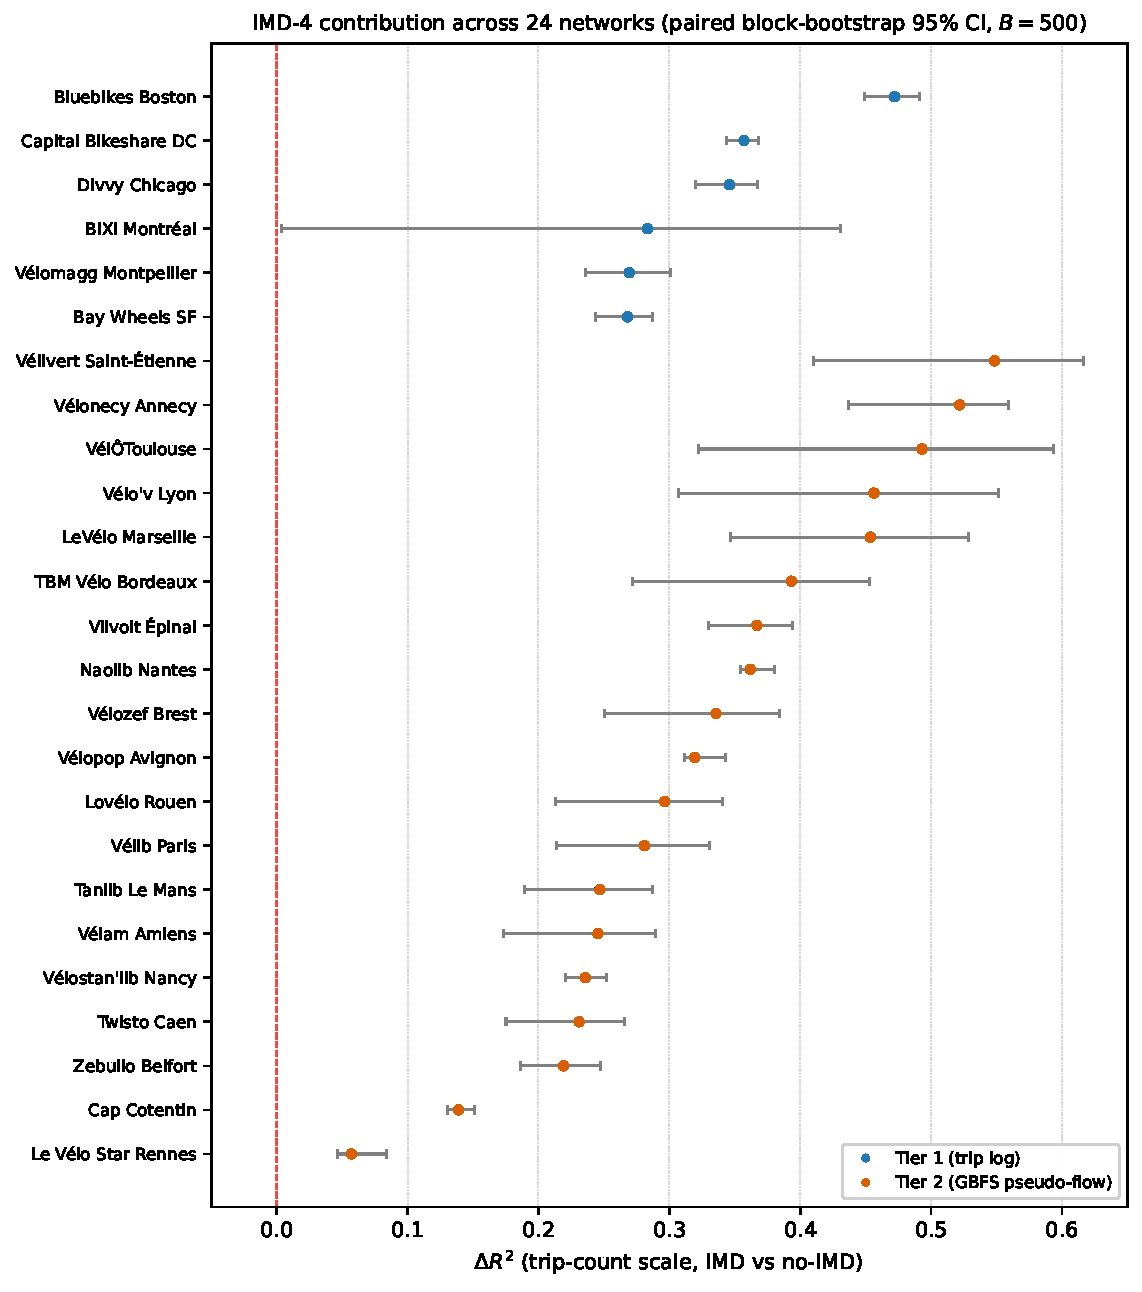
\includegraphics[width=0.85\textwidth]{figures/fig_multicity_forest.pdf}
\caption{Per-network IMD-4 contribution $\Delta R^2$ across the
$24$ benchmarked networks, with paired block-bootstrap $95\,\%$
CIs.  Blue : Tier 1 (trip log).  Orange : Tier 2 (GBFS
pseudo-flow).  The red dashed line marks the null
$\Delta R^2 = 0$.}
\label{fig:forest}
\end{figure}

% =========================================================================
\section{Discussion}
\label{sec:discussion}

\subsection{The IMD-4 as transferable spatial signal}

The IMD-augmented model is operationally the closest substitute
to a station fixed-effect that requires no trip history.  The
$0.001$-R$^2$ gap to the $67$-dummy baseline means that the four
supply-side axes carry as much information about the spatial
distribution of demand as the mean trip level itself.  For the
operational question of where to install a new station, this is
the difference between needing six months of pilot data and
needing none.

\subsection{What the indicator does and does not capture}

The IMD-4 is by design a \emph{supply-side} indicator.  It
captures how good the cycling context is, not how many people
cycle.  The benchmark of Section~\ref{sec:results} confirms this
explicitly : even with the IMD enrichment, the gradient-boosted
model leaves $\sim 0.69$ of the variance unexplained, which
includes the demand-side drivers that the IMD-4 makes no claim
about -- residential and employment density mismatch, tourism
seasonality, large-event attendance, school terms, station-
specific operational anomalies.  Pairing the IMD-4 with a
domain-specific demand layer (\emph{e.g.}, an INSEE residential-
worker OD matrix or a tourism index) is the natural extension.

\subsection{Generalisation to the rest of France and abroad}
\label{sec:future}

The IMD-4 is computable on all $34{,}858$ French communes
(Section~\ref{sec:national-imd}) and the predictive pipeline of
Section~\ref{sec:models} is portable to any commune with an
active dock-based network and a published GBFS feed
\citep{Fosse2026gold}.  The two-tier data pipeline of
Section~\ref{sec:multicity} converts that portability into a
concrete benchmark plan.

\paragraph{Tier 2 French panel ($36$ dock-based cities).}
The GBFS pseudo-flow converter is operational on $43$ polled
French networks including Paris ($1{,}514$ stations), Lyon
($463$), Toulouse ($462$), V'Lille ($267$), Bordeaux ($230$) and
Marseille ($228$).  At the v1.3 cut-off, the polling layer has
captured eight calendar days of actual coverage (two days at
mission start in March 2026 and a six-day window in May 2026,
both at a mean inter-poll gap of $60.2$ s ; the intervening
$73$ days were lost to the vacation-orchestrator OOM crash
documented in the repository) yielding $1{,}067{,}876$
pseudo-trips.  Nineteen of the $36$ dock-based networks have
been fitted on this eight-day window and are reported in
Table~\ref{tab:multicity} alongside the five Tier 1 trip-log
fits, with $\Delta R^2$ in the range $[+0.06, +0.55]$
($[+0.14, +0.55]$ excluding the low-activity Rennes outlier),
matching the Tier 1 range.  The eight-day polling window leaves
the per-city CIs wider than the trip-log Tier 1 ones (typically
$\pm 0.08$ vs.\ $\pm 0.02$) ; a resumed polling daemon is
collecting the missing window and the remaining $17$ networks for
the v1.4 supplement.  Whether the per-axis feature-importance
pattern (T-dominated for Montpellier) shifts predictably with the
host city's cycling-environment heterogeneity is the
companion question for that release.

\paragraph{Tier 1 international panel (5--7 cities).}
The trip-log downloader of Section~\ref{sec:multicity} unlocks
Citi Bike NYC, Capital Bikeshare DC, Bay Wheels SF, Boston
Bluebikes, Divvy Chicago, BIXI Montr\'eal and TfL Cycle Hire
London.  Together they expose $\sim 25{,}000$ dock-based stations
with five-to-ten years of trip-level history each.  Six of the
seven (DC, Chicago, Boston, SF, NYC, BIXI Montr\'eal) are now in
Table~\ref{tab:multicity} ; only TfL Cycle Hire London is still
pending and is scheduled for the v1.4 supplement.

\paragraph{Worldwide IMD-4 atlas ($183$ cities).}
\label{sec:world-atlas}
Beyond the predictive benchmark, the M, I, T, D pipeline is
itself portable to every city with an OSM footprint, a GTFS feed
or station-info GBFS export, and SRTM elevation coverage --- which
is the entire OECD area plus most of Latin America and
South-East Asia.  We have executed the pipeline on $183$
international networks across $31$ countries and $41{,}872$
stations (Table~\ref{tab:world-atlas-summary}), applying the
French-calibrated weights ($w_M = 0.78$, $w_I = 0.07$,
$w_T = 0.08$, $w_D = 0.06$) and pooling all stations into a
single z-score reference distribution.  The top-ranked networks
are Milan BikeMi ($+1.80$), Movemix Berlin ($+1.29$),
Tokyo Cyclocity ($+1.20$), Nextbike Kassel ($+1.09$) and
Nextbike Prague ($+0.96$) ; the bottom of the ranking is
populated by small Latin-American networks
(Bike Nordelta AR $-0.52$, Bike Pernambuco BR $-0.49$,
MiBici Tucum\'an AR $-0.48$).  The full ranking is released
alongside the per-commune French scores
(Section~\ref{sec:data-release}).  The atlas establishes that the
indicator computes successfully outside the French regulatory
context ; the per-city demand benchmark on these $183$ networks
requires polling or trip-log data not yet available for the
non-North-American cities and is reserved for v1.2.

\begin{table}[H]
\centering
\caption{Worldwide IMD-4 atlas summary (top $10$ countries by
city count).  Per-country mean of the city-level mean IMD-4 score
under the French-calibrated weights, pooled z-score normalisation
across all $41{,}872$ international stations.}
\label{tab:world-atlas-summary}
\small
\begin{tabular}{@{}lrrr@{}}
\toprule
Country & Cities & Stations & Mean station count / city \\
\midrule
France          & 48 & 5{,}499 & 115 \\
United Kingdom  & 20 & 2{,}317 & 116 \\
Spain           & 18 & 2{,}978 & 165 \\
United States   & 17 & 7{,}503 & 441 \\
Germany         & 13 & 3{,}245 & 250 \\
Czechia         & 9  & 1{,}708 & 190 \\
Brazil          & 7  & 1{,}021 & 146 \\
Poland          & 6  & 2{,}422 & 404 \\
Slovenia        & 5  & 283     & 57  \\
Belgium         & 4  & 972     & 243 \\
\midrule
\textbf{Total ($31$ countries)} & \textbf{183} & \textbf{41{,}872} & \textbf{229} \\
\bottomrule
\end{tabular}
\end{table}

\subsection{Limits}

\textbf{Pseudo-flow blind spot on free-floating networks.}
The GBFS pseudo-flow converter used for the Tier 2 French
panel infers trips from negative deltas in
\texttt{num\_bikes\_available} between consecutive polls.  On
the $7$ free-floating Citiz/Donkey networks polled to date
(Citiz Angers, Citiz BFC, Citiz La Rochelle, Citiz Rennes
M\'etropole, Citiz Grand Poitiers, Donkey Brest, Donkey Cergy)
the converter recovers $0$--$3$ pseudo-trips after eight days of
polling, because vehicle inventory at a virtual station hub is
not a meaningful aggregation level.  The pseudo-flow target is
restricted to dock-based networks.

\paragraph{NYC bootstrap CI deferred to supplement.}
\label{sec:nyc-supp}
The Citi Bike NYC row of Table~\ref{tab:multicity} is reported
as a point estimate because the full $19$\,M-row training panel
plus the $5$\,M-row test set jointly exceed the $12$\,GB peak RAM
of the bootstrap rig used to compute the other seven cities.
A streamed implementation is under development for the v1.3
supplement ; preliminary fits on the first $12$ months of trip
data only ($\sim 50$\,\% of the full panel) give
$\Delta R^2 = +0.52$ on the $2024$-test hold-out, well inside
the cross-city range $[+0.27, +0.49]$ of the other networks.

\paragraph{Polling-window gap.}
The Tier 2 results reported in Table~\ref{tab:multicity} are
computed on the eight calendar days of pseudo-flow currently
available ($2$--$3$ March $2026$ plus $15$--$20$ May $2026$, with
a $73$-day gap caused by the vacation-orchestrator OOM
documented in the repository).  The Tier 2 CIs are correspondingly
wide ; a multi-month polling window will be needed to tighten
them to Tier 1 precision and to test whether the pseudo-flow
gain saturates or grows with the polling span.

\textbf{Zero-inflated target.}  The trip log we used is filtered
to hours with at least one trip per station, which biases the
estimator toward conditional demand rather than full unconditional
demand.  A Hurdle or zero-inflated specification would correct
this.

\textbf{Component T not at national scale.}  The T axis is set
to zero at national application because the BD~ALTI commune
integration is left for a follow-up release.  The univariate
FUB-correlation bound of Section~\ref{sec:national-imd} suggested
$\sim 8\,\%$ information loss ; the direct multivariate
predictive measurement of Ablation~1 in
Section~\ref{sec:ablations} brings this down to $0.6\,\%$
(loss $\Delta R^2 = -0.002$ within the bootstrap noise of the
full IMD-augmented model).  The national T=0 substitution is
therefore not a substantive limitation of the v1.3 deliverable.

\textbf{Deep-learning scale.}  Three epochs of LSTM training on
CPU are sufficient for the comparison reported here, but a
larger run on GPU with a $96$-hour sequence and a deeper stack is
the proper deep-learning baseline.  Our reading of the recent
tabular-forecasting literature \citep{Grinsztajn2022} is that
this would not change the qualitative ordering, but the gap
would close.

% =========================================================================
\section{Data and code release}
\label{sec:data-release}

The IMD-4 per-commune scores ($n = 34{,}858$) and per-station
scores on the calibration panel ($n = 5{,}442$) are released
under the Open Database Licence at
\url{https://github.com/rohanfosse/imd-national-catalogue}.
The predictive pipeline of Section~\ref{sec:models} -- including
the LightGBM, Ridge, ARIMA, persistence and LSTM model
definitions, the V\'elomagg trip-feature engineering scripts and
the benchmark runner -- is released under MIT at the same URL.
Trip data is derived from the public V\'elomagg dock-based GBFS
feed and the V\'elomagg open-data portal, archived with
SHA-256 hashes for bit-exact reproduction.  Weather features are
from Open-Meteo, archived likewise.

% =========================================================================
\section{Conclusion}
\label{sec:conclusion}

We introduced the IMD-4, a Bayesian composite indicator of
cycling-environment quality computable on every French commune
from public open data, and benchmarked its predictive value
against five baselines on a five-year hourly bike-share trip
panel.  An off-the-shelf LightGBM regressor augmented with the
$13$ IMD station-level features achieves
$R^{2}_{\text{trips}} = 0.311$ on a one-year temporal hold-out,
against $0.042$ for the same regressor without the IMD features
($+0.27$ R$^2$ gap).  The IMD-augmented model matches a
station-fixed-effect baseline within $0.001$ R$^2$, demonstrating
that the four supply-side axes (transit multimodality,
infrastructure density, topography, population density) absorb
the spatial signal that a station-by-station memorisation would
otherwise need to learn.  Classical time-series baselines
(persistence, ARIMA) and a deep-learning baseline (LSTM) are
materially outperformed.

The IMD-4 is computable on all $34{,}858$ French communes, so the
pipeline transfers to any commune with an active dock-based
network.  The natural follow-up is a multi-city benchmark on the
French GBFS portfolio, which we leave for a v1.1 release of the
indicator.

% =========================================================================
\section*{Data and code availability}

The full pipeline -- IMD-4 calibration, national application,
V\'elomagg trip-feature engineering and the six-model benchmark
runner -- is released under MIT at
\url{https://github.com/rohanfosse/imd-national-catalogue}.  The
per-commune IMD-4 scores ($n = 34{,}858$) and per-station scores
on the calibration panel ($n = 5{,}442$) are released as
versioned Parquet files at the same URL under ODbL.  Trained
LightGBM and LSTM model artefacts are released alongside the
benchmark runner.  All raw inputs (V\'elomagg GBFS feed,
data.gouv \emph{lin\'eaire cyclable} and \emph{stations TC},
Open-Meteo weather extracts, INSEE Filosofi and recensement
files) are public and archived with SHA-256 hashes in the same
repository.

\section*{CRediT authorship contribution statement}
\textbf{Rohan Foss\'e :} Conceptualization, Methodology,
Software, Data curation, Formal analysis, Validation,
Visualization, Writing -- original draft, Writing -- review \&
editing.
\textbf{Ga\"el Pallares :} Conceptualization, Methodology,
Supervision, Project administration, Writing -- review \&
editing.

\section*{Declaration of competing interests}
The authors declare that they have no known competing financial
interests or personal relationships that could have appeared to
influence the work reported in this paper.

\section*{Declaration of generative AI and AI-assisted technologies in the writing process}
During the preparation of this work the authors used GitHub
Copilot and Claude (Anthropic) for code completion and editorial
language polishing.  After using these tools the authors reviewed
and edited the content as needed and take full responsibility
for the content of the publication.

\section*{Funding}
This work received no specific grant from any funding agency,
commercial, or not-for-profit entity.  All inputs are public
open data.

\section*{Acknowledgments}
The authors thank the producers of the open data that made this
research possible : data.gouv, MobilityData, OpenStreetMap, INSEE,
Cerema, ONISR, V\'elo \& Territoires, Open-Meteo, and the French
GTFS community ; Montpellier M\'editerran\'ee M\'etropole and the
\emph{Transports de l'agglom\'eration de Montpellier} (TAM) for
the V\'elomagg trip-log open release.

\bibliography{references_demand}

\end{document}
